%Preambule
\documentclass[11pt, a4paper]{article}
\usepackage{geometry}
\geometry{margin=2.5cm}
\usepackage{graphicx}
\usepackage{caption}
\usepackage{subcaption}
\usepackage{booktabs}
\usepackage{listings}
\usepackage{xcolor}
\usepackage{amsmath}
\usepackage{amssymb}
\usepackage{amsfonts}
\usepackage{bm}
\usepackage[T1]{fontenc}
\usepackage[utf8]{inputenc}
\usepackage{float}
\lstset{
    inputencoding=utf8,
    extendedchars=true
}
\lstdefinestyle{matlab}{
  language=Matlab,
  basicstyle=\ttfamily\small,
  keywordstyle=\color{blue},
  commentstyle=\color{green!50!black},
  stringstyle=\color{red},
  numbers=left,
  numberstyle=\tiny,
  stepnumber=1,
  numbersep=5pt,
  frame=single,
  breaklines=true,
  showstringspaces=false
}

%Debut du document
\begin{document}

\begin{titlepage}
\thispagestyle{empty}
    \centering

    \vspace*{2cm}

    {\Large \textbf{\textsc{Polytechnique Montréal}}}\\[0.5cm]
    {\large \textsc{Département de Génie électrique}}\\[2cm]

    {\huge \bfseries ELE2200 - Système et Simulation}\\[0.5cm]
    {\huge \textbf{Devoir 3 (Hiver 2026)}}\\[2cm]

    {\large
\begin{tabular*}{\textwidth}{@{}l@{\extracolsep{\fill}}r@{}}
Costa Alfonso Diego & Matricule : 2374165 \\
Gagnon Louis     & Matricule : 2295595
\end{tabular*}
}\\[2cm]
	{\Large \textbf{Date de remise:} 21 avril 2026
	}
\end{titlepage}

\tableofcontents
\newpage 
\section*{1. Étude du modèle avec contrôleur PID}
\addcontentsline{toc}{section}{1. Étude du modèle avec contrôleur PID}
\subsection*{a) Schémas Simulink}
\addcontentsline{toc}{subsection}{a) Schémas Simulink}
Nous avons créé les schémas simulink suivants:
\begin{figure}[h]
\centering
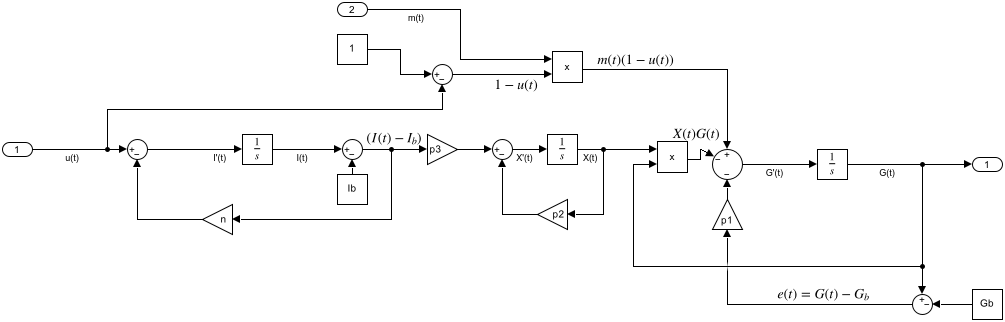
\includegraphics[scale=0.75]{BergmanInOut_incomplet.png}
\caption{Schéma Simulink du système en boucle ouverte}
\end{figure}
\begin{figure}[h]
\centering
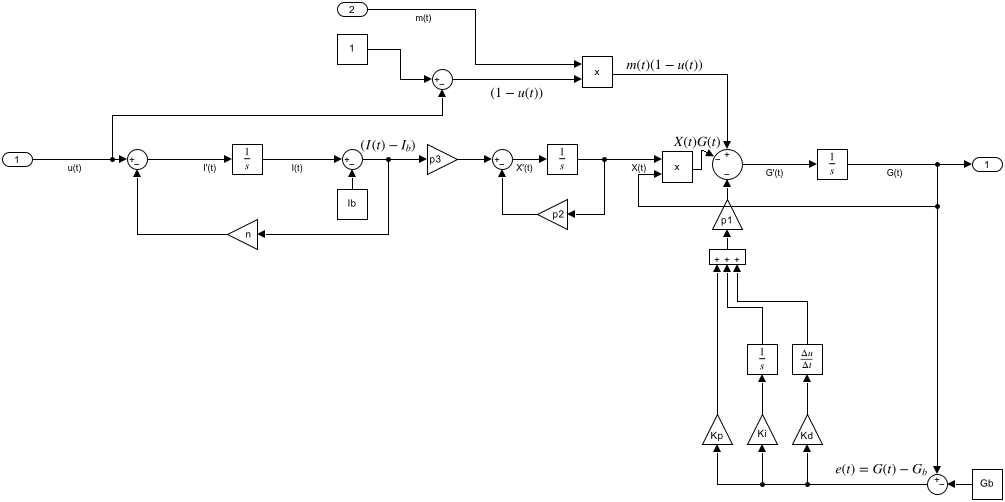
\includegraphics[scale=0.75]{BergmanInOutBF_incomplet.png}
\caption{Schéma Simulink du système en boucle fermée}
\end{figure}
\subsection*{b) Équilibre en boucle ouverte}
\addcontentsline{toc}{subsection}{b) Équilibre en boucle ouverte}
Pour trouver le point d'équilibre du système en boucle ouverte, nous avons écrit le script matlab suivant: 
\begin{lstlisting}[style=matlab]
% Declaration des variables utilisees dans simulink
p1 = 0.03;
p2 = 0.02;
p3 = 1.06*(10^-5);
n = 0.3;
Gb = 92;
Ib = 7.3;
% Conditions initiales 
x0 = [92; 0; 7.3];
u0 = [0; 0];
[x_BO, u_BO, y_BO, dx_BO] = trim("BergmanInOut_incomplet", x0, u0)
\end{lstlisting}
En exécutant le script matlab ci-dessus, on obtient le point d'équilibre suivant:
\begin{center}
$\vec{x}_e=\begin{pmatrix}
G_e \\
X_e \\
I_e \\
\end{pmatrix}=
\begin{pmatrix}
46 \\
0.0024 \\
11.7574 \\
\end{pmatrix}$; $\vec{u}_e=\begin{pmatrix}
u_e \\
m_e \\
\end{pmatrix}=\begin{pmatrix} 
1.3372 \\
3.7701 \\
\end{pmatrix}$ et $y_e=G_e=46$
\end{center}
\subsection*{c) Équilibre en boucle fermée}
\addcontentsline{toc}{subsection}{c) Équilibre en boucle fermée}
Pour trouver le point d'équilibre du système en boucle fermée, nous avons écrit le script matlab suivant:
\begin{lstlisting}[style=matlab]
% On suppose que les valeurs des constantes du PID sont les suivantes
Kp = 0.5;
Kd = 0.01;
Ki = 0.1;
% Conditions initiales 
x0 = [92; 0; 7.3; 0];   % Une condition initiale de plus pour l'integrateur du PID
u0 = [0; 0];
[x_BF, u_BF, y_BF, dx_BF] = trim("BergmanInOutBF_incomplet", x0, u0)
\end{lstlisting}
En exécutant le script matlab ci-dessus, on obtient le point d'équilibre suivant (retourné par trim()):\newline 
\begin{center}
$\vec{x}_e=\begin{pmatrix}
G_e \\
X_e \\
I_e \\ 
\end{pmatrix}=
\begin{pmatrix}
92 \\
-0.0035 \\
0.6241 \\
\end{pmatrix}$; $\vec{u}_e=\begin{pmatrix}
u_e \\
m_e \\
\end{pmatrix}=\begin{pmatrix}
-2.0028 \\
-0.1083 \\
\end{pmatrix}$; $y_e=92$
\end{center}
La fonction trim() a également retourné la valeur d'équilibre pour l'intégrateur du PID, qui est de 0.0076.
\subsection*{d) Fonctions de transfert en boucle ouverte}
\addcontentsline{toc}{subsection}{d) Fonctions de transfert en boucle ouverte}
Pour trouver les fonctions de transfert $G_u$ et $G_m$ en boucle ouverte (autour du point d'équilibre trouvé en b), nous avons écrit le script matlab suivant:
\begin{lstlisting}[style=matlab]
[A_BO, B_BO, C_BO, D_BO] = linmod("BergmanInOut_incomplet", x_BO, u_BO);  % Linearisation
ModEtat_BO = ss(A_BO, B_BO, C_BO, D_BO);   % Creer un modele d'etat 
FT_BO = tf(ModEtat_BO)                     % Extraire les fonctions de transfert du modele d'etat
Gu_BO = minreal(FT_BO(1))                  % Gu(s) en boucle ouverte 
Gm_BO = minreal(FT_BO(2))                  % Gm(s) en boucle ouverte
\end{lstlisting}
En exécutant le script matlab ci-dessus, on obtient les fonctions de transfert suivantes: 
$$\boxed{G_{u_{BO}}(s)=\frac{-3.77s^2-1.206s-0.02311}{s^3+0.3524s^2+0.01636s+0.0001942}}$$
$$\boxed{G_{m_{BO}}(s)=\frac{-0.3372}{s+0.03236}}$$
\subsection*{e) Fonctions de transfert en boucle fermée et pôles}
\addcontentsline{toc}{subsection}{e) Fonctions de transfert en boucle fermée et pôles}
Pour trouver les fonctions de transfert $G_u$ et $G_m$ en boucle fermée (autour du point d'équilibre trouvé en c) ainsi que les pôles du système en boucle ouverte et fermée, nous avons écrit le script matlab suivant:
\begin{lstlisting}[style=matlab]
[A_BF, B_BF, C_BF, D_BF] = linmod("BergmanInOutBF_incomplet", x_BF, u_BF); % Linearisation
ModEtat_BF = ss(A_BF, B_BF, C_BF, D_BF);  % Creer un modele d'etat 
FT_BF = tf(ModEtat_BF)                     % Extraire les fonctions de transfert du modele d'etat
Gu_BF = minreal(FT_BF(1))                  % Gu(s) en boucle fermee
Gm_BF = minreal(FT_BF(2))                  % Gm(s) en boucle fermee
eig(A_BO)                 % Poles du systeme en boucle ouverte
eig(A_BF)                 % Poles du systeme en boucle fermee
\end{lstlisting}
En exécutant le code matlab ci-dessus, on obtient les fonctions de transfert en boucle fermée suivantes:
$$\boxed{G_{u_{BF}}(s)=\frac{0.1083s^3+0.03467s^2-0.0003252s+1.371\times 10^{-23}}{s^4+0.3315s^3+0.01267s^2+0.001029s+1.8\times 10^{-5}}}$$
$$\boxed{G_{m_{BF}}(s)=\frac{3.003s}{s^2+0.01146s+0.003}}$$ 
les pôles du système linéarisé en boucle ouverte: 
$$\begin{cases}
p_0 = -0.0324\\
p_1 = -0.02\\
p_2 = -0.3
\end{cases}$$
ainsi que les pôles du système linéarisé en boucle fermée:
$$\begin{cases}
p_0 = -0.0057+0.0545i\\
p_1 = -0.0057-0.0545i\\
p_2 = -0.02\\
p_3 = -0.3
\end{cases}$$
\subsection*{f) Stabilité pour un correcteur proportionnel}
\addcontentsline{toc}{subsection}{f) Stabilité pour un correcteur proportionnel}
En utilisant seulement $G_{u_{BO}}(s)$ trouvée auparavant, on peut schématiser le système linéarisé en boucle fermée comme suit:
\begin{figure}[h]
\centering
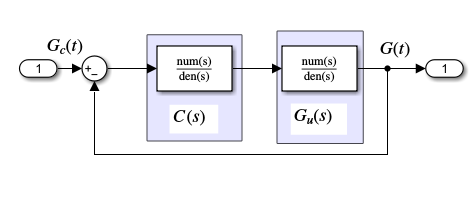
\includegraphics[scale=0.75]{Schema_commande.png}
\caption{Diagramme fonctionnel du système \underline{linéarisé} en boucle fermée}
\end{figure} \\
Il s'agit d'une simple contre-réaction négative dont la fonction de transfert est:
$$\frac{G(s)}{R(s)}=\frac{C(s)G_{u_{BO}}(s)}{1+C(s)G_{u_{BO}}(s)}$$
En utilisant $G_{u_{BO}}(s)$ trouvée précédemment ainsi que $C(s)=K_p$, on trouve la forme suivante:
$$\frac{K_p(-3.77s^2-1.206s-0.02311)}{s^3+(0.3524-3.77K_p)s^2+(0.01636-1.206K_p)s+(0.0001942+0.02311K_p)}$$
On doit donc faire l table de Routh-Hurwitz pour le polynôme du dénominateur, qui est:
$$p(s)=s^3+(0.3524-3.77K_p)s^2+(0.01636-1.206K_p)s+(0.0001942+0.02311K_p)$$
On pose 
$$\begin{cases}
a_3 = 1\\
a_2 = (0.3524-3.77K_p)\\
a_1 = (0.01636-1.206K_p)\\
a_0 = (0.0001942-0.02311K_p)
\end{cases}$$
et on effectue la table de Routh-Hurwitz, i.e.: \newline
\begin{center}
\renewcommand{\arraystretch}{1.5}
\begin{tabular}{|c||c|c|c|}

\hline
 $s^3$ & $a_3$ & $a_1$  & $0$ \\
\hline
 $s^2$ & $a_2$ & $a_0$ & $0$ \\
\hline
 $s^1$ & $-\frac{\begin{vmatrix}
a_3 & a_1 \\
a_2 & a_0
\end{vmatrix}}{a_2}=b_1$ & $0=b_2$ & $0$ \\
\hline
 $s^0$ & $-\frac{\begin{vmatrix}
a_2 & a_0 \\
b_1 & b_2
\end{vmatrix}}{b_1}=c_1$ & $0$ & $0$ \\
\hline
\end{tabular}
\end{center}
On développe les coefficients $b_1$ et $b_2$: 
$$b_1=\frac{(0.01636-1.206K_p)(0.3524-3.77K_p)-(0.0001942-0.02311K_p)}{(0.3524-3.77K_p)}$$
$$c_1=a_0=(0.0001942-0.02311K_p)$$
Ensuite, on applique le critère de Routh-Hurwitz, i.e. que l'on impose que les coefficients $a_3$, $a_2$, $b_1$ et $c_1$ doivent être strictement supérieurs à 0 pour que le polynôme identifié précédemment soit stable. On sait que $a_3=1$, donc strictement positif pour tout $K_p$. Ensuite, la condition sur $a_2$:
$$a_2 > 0 \Leftrightarrow 0.3524-3.77K_p > 0 \Leftrightarrow \boxed{K_p < 0.09347}$$
Ensuite, la condition sur $b_1$:
$$b_1 > 0 \Leftrightarrow (0.01636-1.206K_p)(0.3524-3.77K_p)-(0.0001942-0.02311K_p) > 0$$
$$\Leftrightarrow 4.54662K_p^2-0.4635616K_p+0.005571064 > 0$$
Pour trouver l'intervalle solution, on trouve d'abord les racines du polynôme de gauche:
$$K_{p_{1,2}}=\frac{0.4635616\pm \sqrt{(-0.4635616)^2-4(4.54662)(0.00557)}}{2(4.54662)}$$ $$\Rightarrow K_{p_1}=0.013917 \text{ et } K_{p_2}=0.08803958$$ 
Le polynôme de gauche a une concavité positive (car la dérivée seconde par rapport à $K_p$ est positive), donc l'intervalle solution est:
$$\boxed{K_p \; \epsilon \{-\infty < 0.013917 \cup 0.08803958 < \infty \}}$$
Finalement, la condition sur $c_1$:
$$c_1 = a_0 > 0 \Leftrightarrow (0.0001942-0.02311K_p)>0 \Leftrightarrow \boxed{K_p < 0.008403}$$
Donc, en regroupant les différentes conditions sur $K_p$ vues ci-dessus, la condition finale sur $K_p$ est la suivante:
$$\boxed{K_p < 0.008403}$$
Selon le critère provenant de Routh-Hurwitz établit ci-dessus, le système ne devrait pas être stable pour $K_p=0.5$
\subsection*{g) Lieu des racines et stabilité}
\addcontentsline{toc}{subsection}{g) Lieu des racines et stabilité}
En utilisant la fonction $G_{u_{BO}}(s)$ trouvée auparavant, on écrit le code matlab suivant (les valeurs de gains sont $K_d=0.001$, $K_i=0.1$ et $K_p=0.5$):
\begin{lstlisting}[style=matlab]
% Utiliser rltool pour le lieu des racines
s = tf("s");
Correcteur = -(Kd*(s^2) + Kp*s + Ki)/s;
rltool(Gu_BO, Correcteur)
\end{lstlisting}
En exécutant le code matlab ci-dessus, ceci apparaît:
\begin{figure}[H]
\centering
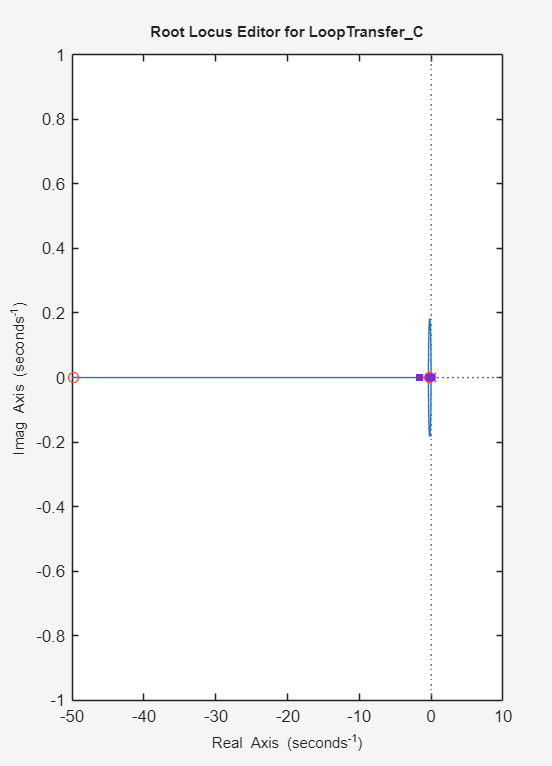
\includegraphics[scale=0.75]{LDR_figure1.png}
\caption{Lieu des racines avec PID, vue globale}
\end{figure}
\begin{figure}[H]
\centering
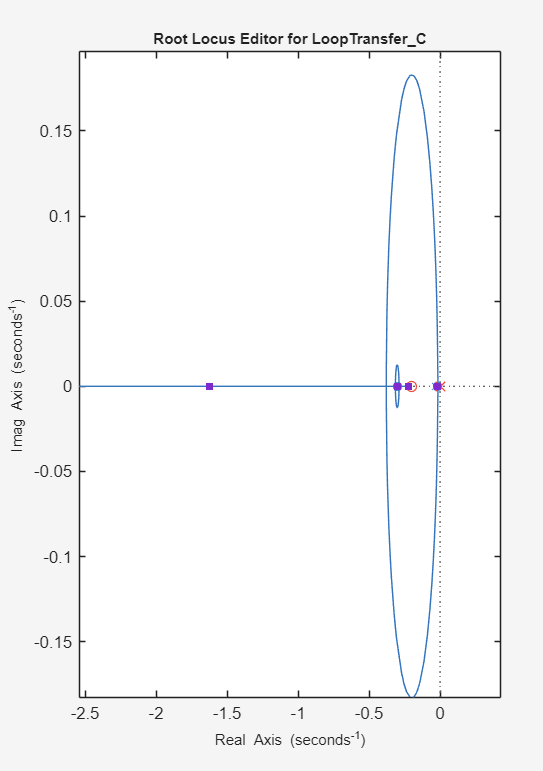
\includegraphics[scale=0.75]{LDR_figure2.png}
\caption{Lieu des racines avec PID, vue agrandie}
\end{figure} 
\noindent On peut voir qu'en utilisant rltool() avec un correcteur PID (avec les valeurs mentionnées dans l'énoncé) multiplié par un signe négatif, le LDR ne dépasse jamais l'axe des imaginaires, donc que le système est stable avec un correcteur $C(s)=-\frac{(0.01s^2+0.5s+0.1)}{s}$
Nous pensons que ce résultat est cohérent avec notre condition trouvée en f), car nous avons essentiellement inséré un PID dans rltool() avec une valeur de $K_p$ négative et que puisque rltool() vérifie le LDR pour $K_p > 0$, alors cela se traduit par le fait que le système est stable pour le nouveau $K_p$ qui est négatif.

\subsection*{h) Erreur en régime permanent} 
\addcontentsline{toc}{subsection}{h) Erreur en régime permanent}
Pour l'erreur en régime permanent du système en boucle fermée, nous avon décidé de faire un schéma simulink suivant:
\begin{figure}[H]
\centering
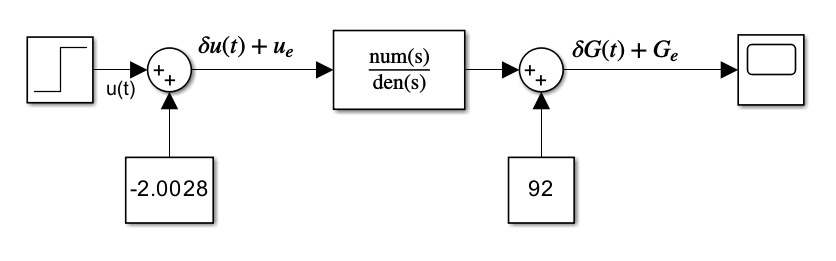
\includegraphics[scale=0.75]{Schema_pourERP.png}
\caption{Schema simulink}
\end{figure}
\noindent Dans ce schéma, le bloc de transfert est 
$G_{u_{BF}}(s)=\frac{0.1083s^3+0.03467s^2-0.0003252s+1.371\times 10^{-23}}{s^4+0.3315s^3+0.01267s^2+0.001029s+1.8\times 10^{-5}}$, l'entrée est la somme de $\delta u(t)=2H_s(t)$ avec la valeur d'équilibre en boucle fermée $u_e=-2.0028$ trouvée en c) et la sortie prélevée par le bloc scope est la somme de la sortie $\delta G(t)$ et la valeur d'équilibre en boucle fermée $G_e = 92$ trouvée en c). Nous avons fait ainsi, car $G_{u_{BF}}$ est une fonction de transfert linéarisée autour d'un point d'équilibre. Donc, si on veut une réponse complète et correcte, il faut inclure les valeurs d'équilibre (d'ou les valeurs d'équilibre ajoutées de par les sommateurs). Ensuite, nous avons écrit le code matlab ci-dessous pour tracer la réponse complète $\delta G(t) + G_e$:
\begin{lstlisting}[style=matlab]
out0 = sim("BF_Q1_ERP.slx", 'Solver','ode45','StopTime','2000');
plot(out0.ERP(:,1), out0.ERP(:,2), "Color","b");
grid on
title("Graphe de G(t) en BF lin\'earis\'e pour $\delta u(t)=2H_s(t)$ et $\delta m(t)=0$", "Interpreter","Latex");
xlabel("temps (s)", "Interpreter","Latex");
ylabel("Glyc\'emie G(t) (mg/dL)","Interpreter","latex");
print -dpng ERP.png;
\end{lstlisting}
pour ensuite l'exécuter, pour obtenir le graphe suivant:
\begin{figure}[H]
\centering
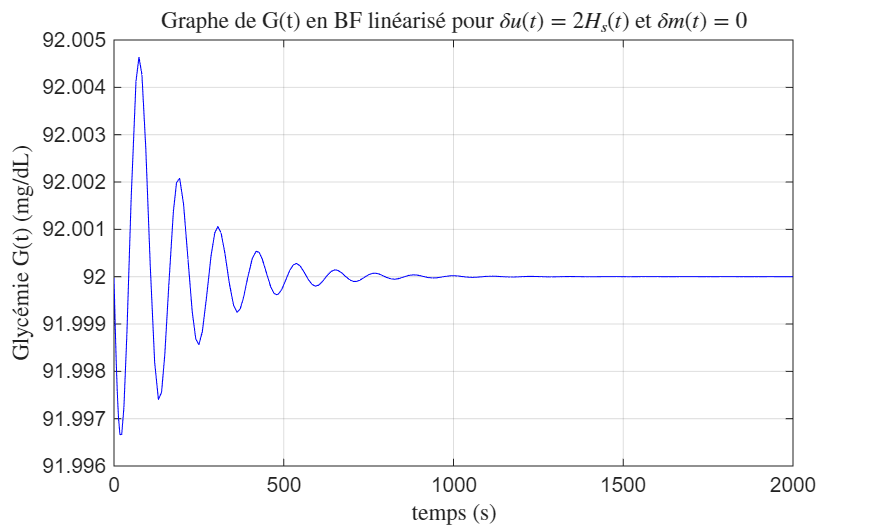
\includegraphics[scale=0.75]{ERP.png}
\caption{Réponse pour calculer l'ERP}
\end{figure}
\noindent On peut voir dans le graphe ci-dessus que la glycémie finit par se stabiliser à 92mg/dL, ce qui est exactement la valeur de $G_b$. Donc, puisque il a été définie dans l'énoncé que $e(t)=G(t)-G_b$, alors l'erreur $e(t)$ lorsque t tend vers l'infini tend vers 0. On peut dire que l'erreur en régime permanent est de 0.

\section*{2. Commande de la glycémie en présence de perturbations}
\addcontentsline{toc}{section}{h) Erreur en régime permanent}
\subsection*{a) Simulation non linéaire sans contrôleur}
\addcontentsline{toc}{subsection}{a) Simulation non linéaire sans contrôleur}
Nous avons fait le schéma simulink suivant:
\begin{figure}[H]
\centering
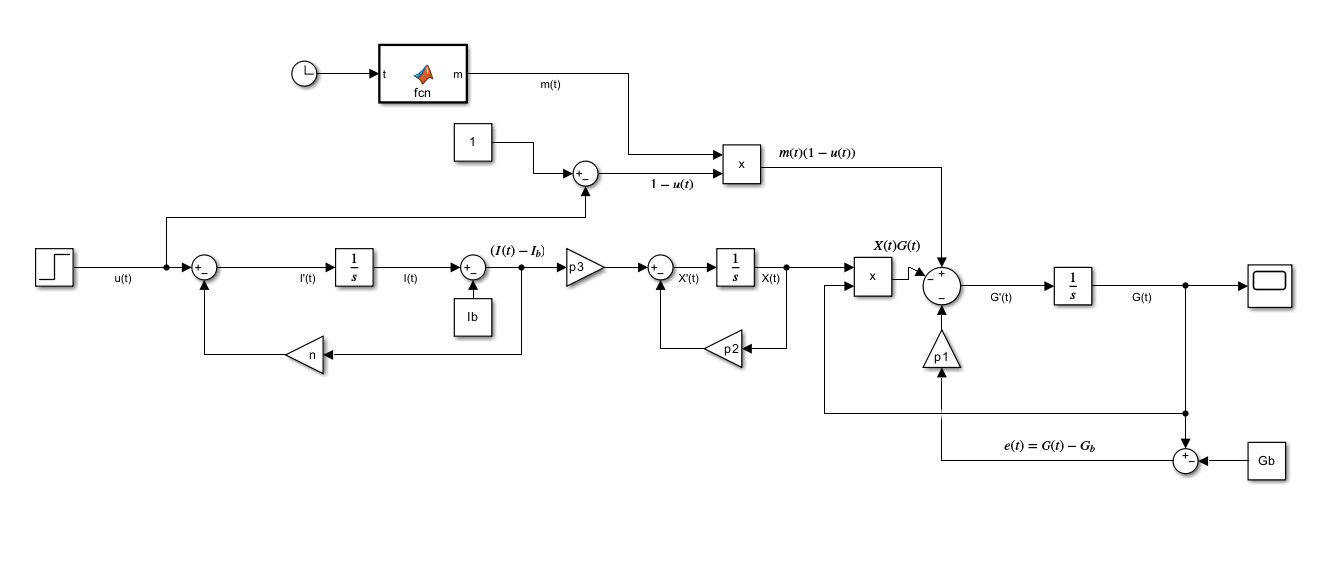
\includegraphics[scale=0.5]{SchemaQ2a.png}
\caption{Diagramme fonctionnel pour a)}
\end{figure}
\noindent Il s'agit du diagramme complété dans la question 1a), mais avec les entrées $u(t)=2H_s(t)$ et $m(t)=5\chi_{[0.5]}(t)$ et un bloc scope pour pouvoir prélever la sortie $G(t)$. Le contenu du bloc "matlab function" est le suivant: 
\begin{lstlisting}[style=matlab]
function m = fcn(t)

if (t <= 0 && t >= 5)
    m = 5*1;

else
    m = 0;
end
\end{lstlisting}
Nous avons ensuite écrit le code matlab suivant pour tracer $G(t)$:
\begin{lstlisting}[style=matlab]
x0 = [92, 0, 7.3];  % conditions initiales
figure(2);
out1 = sim("BO_Q2.slx", 'Solver','ode45','StopTime','400');
plot(out1.GBO_Q2(:,1), out1.GBO_Q2(:,2), "Color","b");
grid on
title("Graphe de G(t) en BO pour u(t)=2$H_s(t)$ et m(t)=$5\chi_{[0,5]}(t)$", "Interpreter","Latex");
xlabel("temps (s)", "Interpreter","Latex");
ylabel("Glyc\'emie G(t) (mg/dL)","Interpreter","latex");
print -dpng Figure1_Q2a.png;
% La glycemie se stabilise dans la zone de securite
\end{lstlisting}
pour ensuite l'exécuter pour obtenir le graphe suivant:
\begin{figure}[H]
\centering
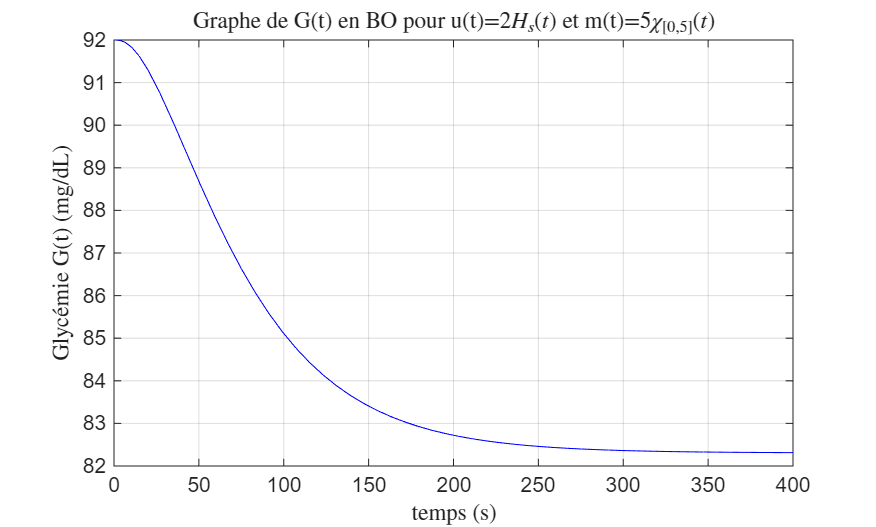
\includegraphics[scale=0.75]{Figure1_Q2a.png}
\caption{Graphe de G(t) en BO}
\end{figure}
\noindent On peut voir dans le graphe ci-dessus que la réponse temporelle G(t) débute à 92 pour ensuite passer par un régime transitoire décroissant, pour ensuite se stabiliser à environ 82.5mg/dL. Cette valeur de glycémie est comprise dans l'intervalle de sécurité $70mg/dL < BG < 180mg/dL$. Donc, oui, la glycémie reste dans la zone de sécurité, mais elle semble se stabiliser en dessous du niveau de glycémie basal qui est de 92mg/dL. Cela n'est pas forcément le meilleur cas de figure. Idéalement, on voudrait que la glycémie se stabilise autour du niveau de glycémie basal (92mg/dL).

\subsection*{b) Simulation non linéaire avec contrôleur}
\addcontentsline{toc}{subsection}{b) Simulation non linéaire avec contrôleur}
Nous avons fait le schéma simulink suivant:
\begin{figure}[H]
\centering
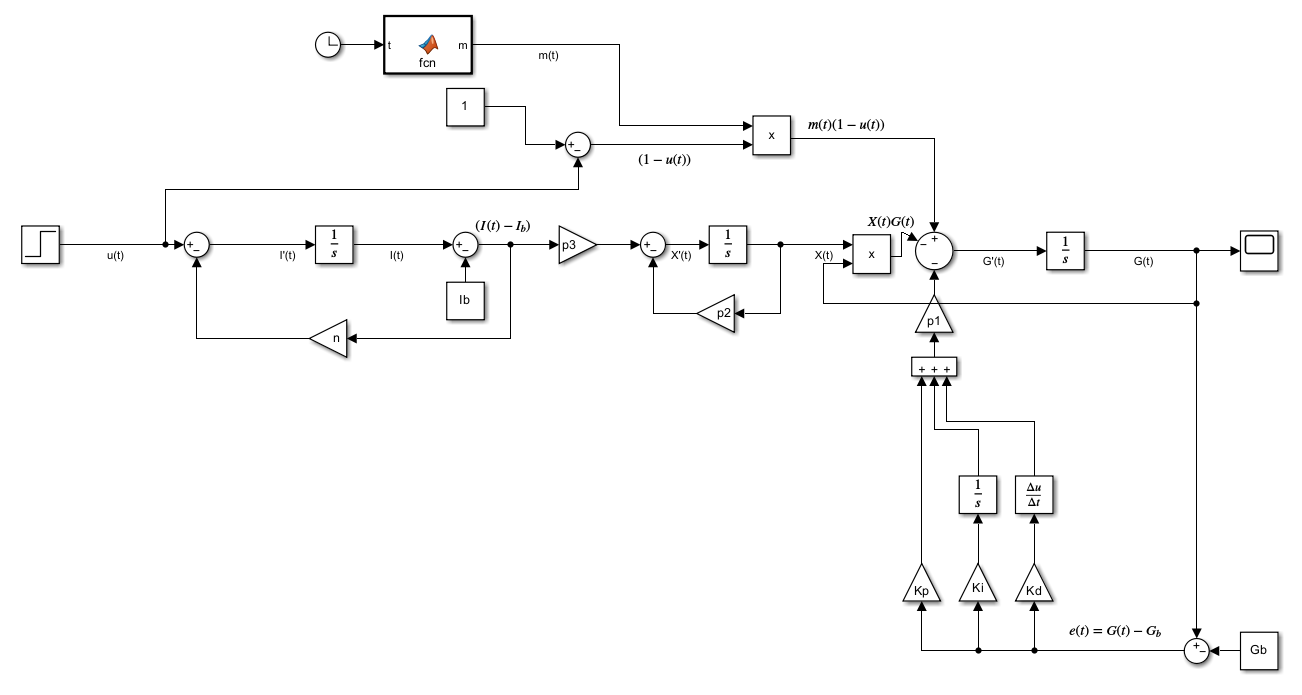
\includegraphics[scale=0.5]{SchemaQ2b.png}
\caption{Diagramme fonctionnel pour b)}
\end{figure}
\noindent Il s'agit du diagramme en boucle fermée complété dans la question 1a), mais avec les entrées $u(t)=2H_s(t)$ et $m(t)=5\chi_{[0.5]}(t)$ et un bloc scope pour pouvoir prélever la sortie $G(t)$. Le contenu du bloc "matlab function" est le même que celui de la question précédente (en a).
Nous avons ensuite écrit le code matlab suivant pour tracer le graphe de $G(t)$ en boucle fermée ainsi qu'un graphe superposant $G(t)$ en boucle ouverte et fermée: \newpage
\begin{lstlisting}[style=matlab]
figure(3);
out3 = sim("BF_Q2.slx", 'Solver','ode45','StopTime','400');
plot(out3.GBF_Q2(:,1), out3.GBF_Q2(:,2), "Color","b");
grid on
title("Graphe de G(t) en BF pour u(t)=2$H_s(t)$ et m(t)=$5\chi_{[0,5]}(t)$", "Interpreter","Latex");
xlabel("temps (s)", "Interpreter","Latex");
ylabel("Glyc\'emie G(t) (mg/dL)","Interpreter","latex");
print -dpng Figure1_Q2b.png;
figure(4);
plot(out1.GBO_Q2(:,1), out1.GBO_Q2(:,2), "Color","b");
hold on
plot(out3.GBF_Q2(:,1), out3.GBF_Q2(:,2), "Color","r");
grid on
title("Graphe de G(t) pour u(t)=2$H_s(t)$ et m(t)=$5\chi_{[0,5]}(t)$", "Interpreter","Latex");
xlabel("temps (s)", "Interpreter","Latex");
ylabel("Glyc\'emie G(t) (mg/dL)","Interpreter","latex");
legend("boucle ouverte", "boucle ferm\'ee","Interpreter", "Latex", "Location","southwest");
print -dpng Figure2_Q2b.png;
\end{lstlisting}
En faisant exécuter le code matlab ci-dessus, on obtient les graphes suivants:
\begin{figure}[H]
\centering
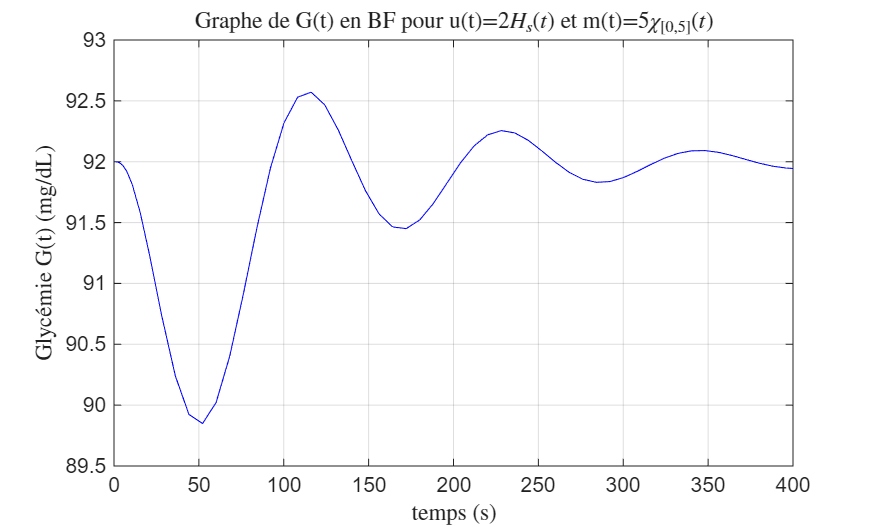
\includegraphics[scale=0.75]{Figure1_Q2b.png}
\caption{Réponse en boucle fermée seulement}
\end{figure}
\begin{figure}[H]
\centering
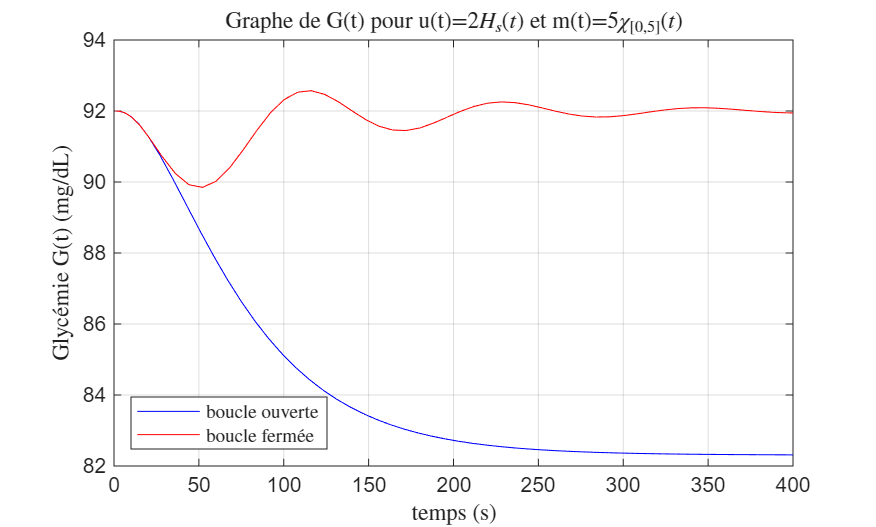
\includegraphics[scale=0.75]{Figure2_Q2b.png}
\caption{Réponses en boucles ouverte et fermée}
\end{figure}
\noindent On observe dans le graphe de la figure 11 que la réponse $G(t)$ débute à 92, passe à travers un régime transitoire oscillatoire (probablement dû à la paire de pôles complexes conjugués) pour ensuite se stabiliser à 92mg/dL (le niveau basal de glycémie $G_b$). La réponse finit donc par se stabiliser directement sur le niveau basal de glycémie $G_b$ qui est bel et bien dans la zone de sécurité. On peut comparer directement les réponses en boucle ouverte et fermée en observant le graphe de la figure 12. On remarque que la réponse en boucle ouverte se stabilise à une glycémie dans la zone de sécurité, certes, mais en-dessous du niveau basal, ce qui peut causer des effets physiologiques non souhaitables. La réponse en boucle fermée, quant à elle, se stabilise directement sur $G_b$, ce qui est nettement plus souhaitable que la valeur en régime permanent en boucle ouverte, car le niveau de glycémie "normal" est exactement 92mg/dL (la valeur optimale pour que l'individu se sente bien, fonctionnement normal du corps reprend). On peut également remarquer que les oscillations dans le régime transitoire de la réponse en boucle fermée ne sortent pas de la zone de sécurité et même qu'elles restent plutôt près de 92mg/dL. Donc, même lorsque la glycémie ne s'est pas encore totalement stabilisée, la réponse en boucle fermée est quand même plus bénéfique que celle en boucle fermée.
\end{document}